%Simulation Results and Discussion


\subsection{Length of shortest tour}

In a first attempt the dependency of the shortest tour length on different parameters is analysed. Thereby the number of completed rounds each agent finishes is varied. Moreover the relative weighting of deposited pheromone and closeness is analysed by changing the parameter \beta and the value of the update rate \alpha is optimized. \\
The shortest tour length is calculated for a 51 cities problem and averaged over 10 trials. In Figure \ref{fig:roundsp} its dependency on the number of completed tours is shown. As expected the average length decreases asymptotically towards the value of the optimal path. This value is then compared to the known solution from \cite{web:data}. This is also done with the trajectory vector of the shortest tour, i.e. the sequence of city numbers which yields the optimal tour.

\begin{figure}[h!]
\begin{center}
\includegraphics[width=11cm, height= 6 cm]{rounds_vs_shortestpath}
\caption{Shortest tour length averaged over 10 runs for different numbers of rounds. The value approximates the optimal solution for \approx 2000 rounds?}
\label{fig:roundsp}
\end{center}
\end{figure}
Figure \ref{fig:alphasp}
\begin{figure}[h!]
\begin{center}
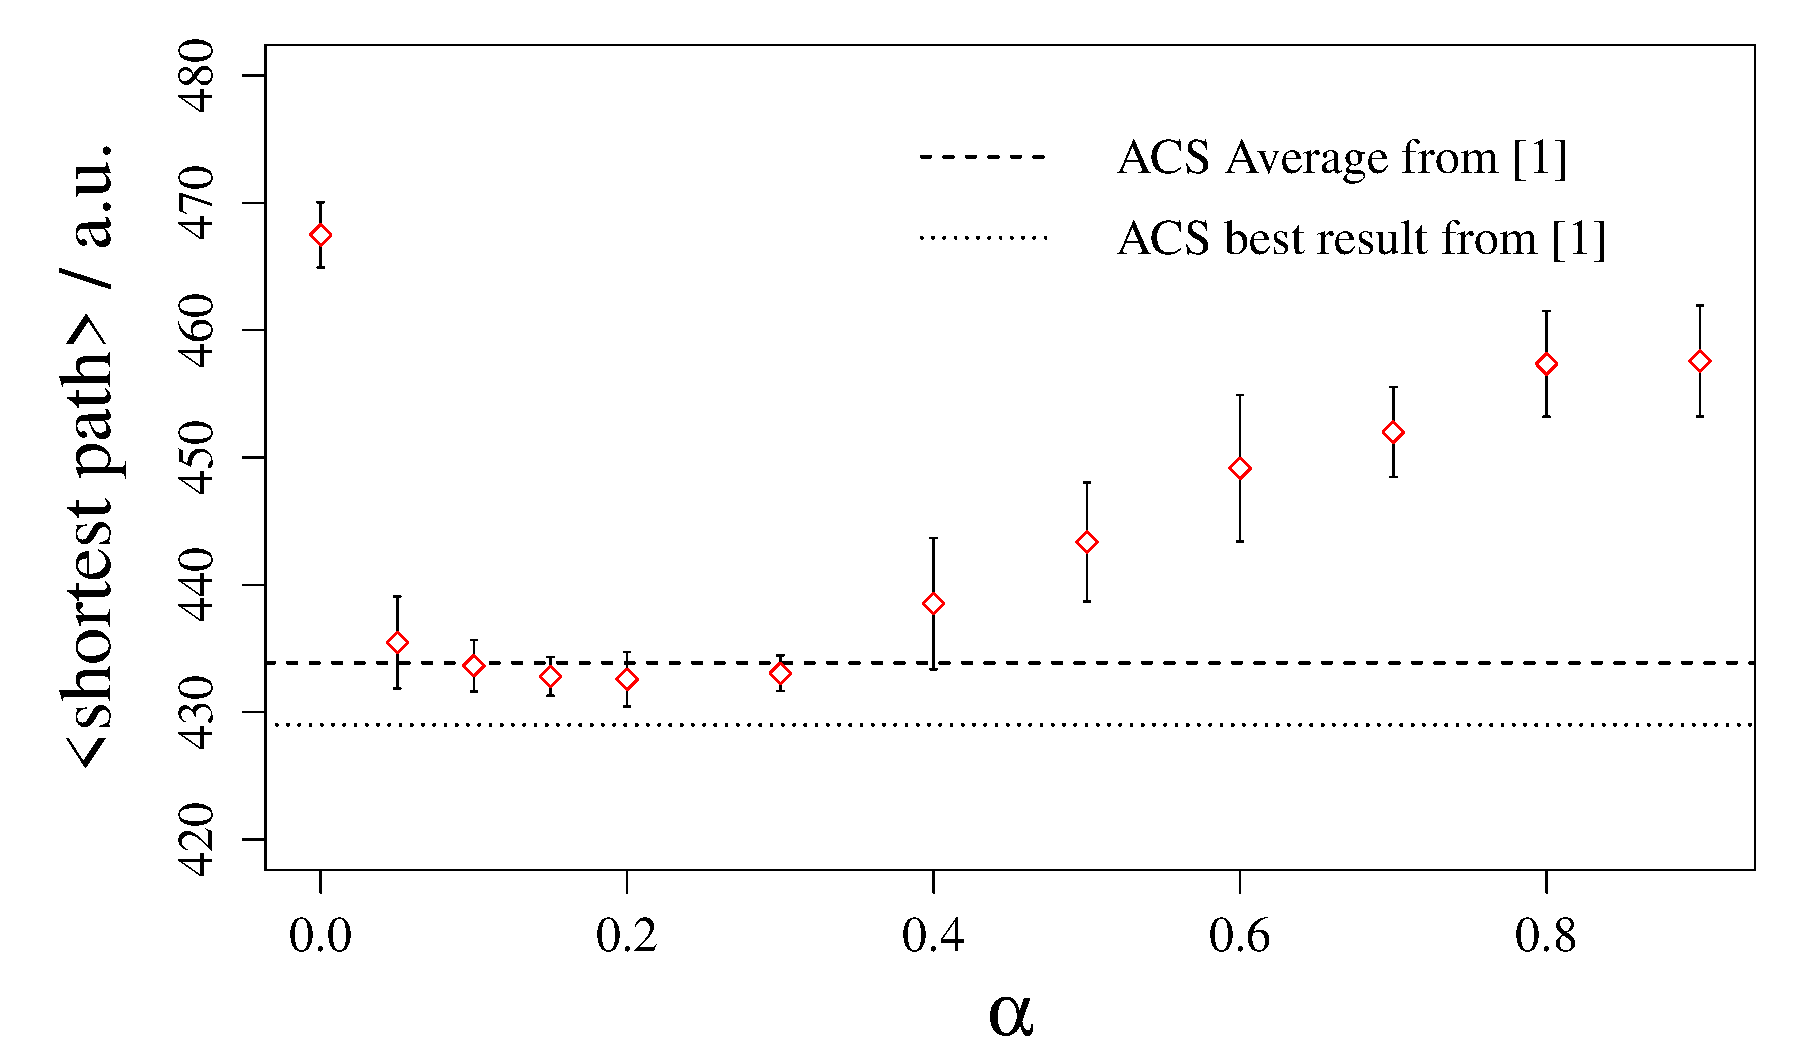
\includegraphics[width=11cm, height= 6 cm]{alpha_vs_shortestpath}
\caption{.}
\label{fig:alphasp}
\end{center}
\end{figure}

\subsection{Model adaptions}

